\documentclass[spanish,12pt,letterpapper]{article}
\usepackage{babel}
\usepackage[utf8]{inputenc}
\usepackage{graphicx}
\usepackage{hyperref}
\begin{document}
	\begin{titlepage}
		\begin{center}
			
\includegraphics[width=0.6\textwidth]{../logoUnADM}~\\[1cm] 
			\textsc{Universidad Abierta y a Distancia de México}\\[0.8cm]
			\textsc{Desarrollo de Software}\\[1.8cm]
			
			\textbf{ \Large Evidencia de Aprendizaje}\\[3cm]
			
			Diego Antonio Plascencia Lara\\ ES1421004131 \\[0.4cm]
			Facilitador(a): Julia Alicia Reyes Rios\\
			Materia: Modelado de Negocios\\
			Grupo: DS-DMDN-1601-B1-007 \\
			Unidad: II \\
			
			\vfill México D.F\\{\today}
			
		\end{center}
	\end{titlepage}
	
	\section{Requerimientos}
	
	``EL ENTRENAMIENTO AUDITIVO INTERACTIVO''\\
	
	``El entrenamiento auditivo de un músico es una de las tareas más importantes para su vida profesional. En su etapa formativa es uno de los aspectos que deberían considerarse prioritarios, sin embargo, esto no necesariamente ocurre. Es una labor tediosa y difícil de llevar a cabo, especialmente en su etapa inicial. Para cubrir esta necesidad primordial, un grupo de maestros de asignaturas teórico musicales decidió plantear un subproyecto PAPIME para la implementación de un Laboratorio de Entrenamiento Auditivo Interactivo en la Escuela Nacional de Música, en donde los estudiantes pudieran acudir a trabajar de forma individual y utilizar programas computacionales que los ayudaran en su entrenamiento auditivo, mejorando la calidad de su formación musical''
	
	\section{Actividades}
	Proceso ``Uso del Laboratorio'':\\
	
	\begin{itemize}
	\item Solicitar el Permiso de Uso del Recurso
	\item Usar Software Correspondiente al Objetivo
	\item Terminar la Practica y Abandonar el Aula
	\item Otorgar Recursos
	\item Verificar el correcto uso de los recursos
	\item Registrar Salidas
	\item Dar mantenimiento al equipo de computo
	\item Atender Solicitudes de Reemplazo de Equipo
	\end{itemize}
	
	\section{Actores}
	\textbf{ALUMNO:\\}	
	Solicitar el Permiso de Uso del Recurso\\
	Usar Software Correspondiente al Objetivo\\
	Terminar la Practica y Abandonar el Aula\\
	
	\textbf{RECEPCIONISTA:\\}	
	Otorgar Recursos\\
	Verificar el correcto uso de los recursos\\
	Registrar Salidas\\
	Dar mantenimiento al equipo de computo\\

	\textbf{DIRECCIÓN GENERAL DE COMPUTO:\\}
	Atender Solicitudes de Reemplazo de Equipo
	
	\subsection{Conexiones}
	El proceso empieza cuando un alumno requiere utilizar el laboratorio.\\
	Solicitar recurso esta conectada a una compuerta condicional, si se identifica el alumno se procede a la tarea ``Usa el Software'', si no se termina el proceso.\\
	La tarea ``Usa el Software`` tiene una conexión de mensaje a ``Registrar entrada'' en el pool ``Auxiliar técnico'', en este pool hasta la tarea ``Registrar salida'' donde regresa un mensaje al Alumno, también en la actividad ``Dar mantenimiento al equipo hay un mensaje bidireccional con la única actividad (``Atender solicitudes de equipo nuevo'') de DGDC.
	
	Por lo que las conexiones de \textbf{mensaje} son entre:

	\begin{itemize}
	 \item \textbf{``Usar el Software'' (alumno) - ``Registrar entrada'' (aux. tec.)} 
	 \item \textbf{``Registrar salida'' (aux. tec.) - ``Terminar sesion'' (alumno)} y 
	 \item \textbf{``Dar mantenimiento al equipo'' (aux. tec.) - ``Atender solicitudes de equipo nuevo'' (dgdc)}
	\end{itemize}
	
	\section{Diagramas BPMN}
	\begin{center}
	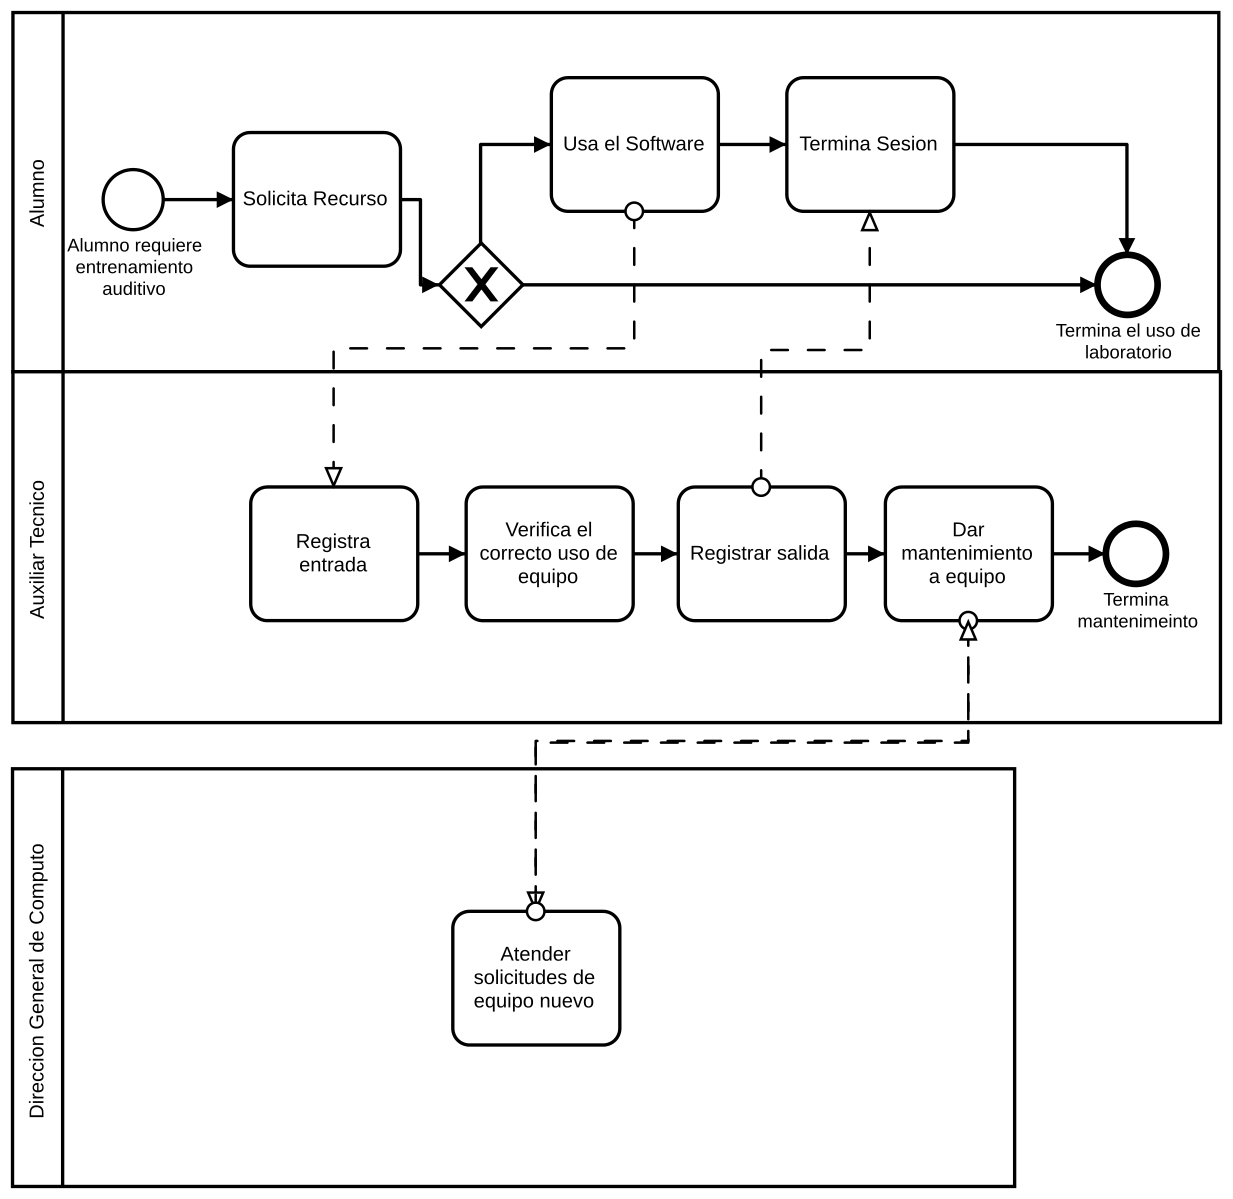
\includegraphics[width=1\textwidth]{./bpmn}~\\[1cm]
	\end{center}
	
	En el diagrama se muestran las tareas principal, divididas por pools que en este caso son las personas o actores (alumno, técnico, la dgdc) que se comunican entre si por medio de vínculos de mensajes. Al final se logra un correcto uso del laboratorio.
	
	\section{Manual}
	\subsection{Proceso del Laboratorio}
	El siguiente manual tiene como fin detallar el proceso de uso del laboratorio de computo para el entrenamiento auditivo en la escuela de Música de la UNAM.\\
	
	Este manual se divide en 3 secciones, las cuales están dirigidos a las diferentes personas que interactúan en el proceso, los cuales uno de ellos es dirigido al alumno que utilizara el sistema de computo y el software de entrenamiento auditivo, otro es dirigido al auxiliar técnico que gestiona y da mantenimiento a los recursos en el laboratorio, y el ultimo esta dirigido a la dirección general de computo, el cual provee los recursos y toma decisiones acerca de modificaciones a el laboratorio.  
	
	\subsection{Manual para el Alumno}
	\textbf{Para ingresar a el laboratorio usted debe:\\}
	1. Solicitar una computadora al auxiliar técnico (AT) en el laboratorio.\\	
	2. El AT le recogerá su identificación escolar y le dará un numero de computadora el cual le fue asignado.\\
	3. Una vez teniendo su numero de maquina, debe pasar al laboratorio y usar la maquina que coincida con su numero dado. Los números de maquina se encuentras sobre de los monitores de estas.\\
	
	\textbf{Para hacer uso de los recursos deberá:\\}
	1. Encender la maquina y entrar en la sesión de ``Invitado''.\\
	2. De la barra de programas o en el Escritorio debe iniciar el programa ``Ear Master School 4.0''\\
	3. En este programa debe seleccionar la sección correspondiente a la indicada por su programa de estudios o profesor.\\
	
	\textbf{Al terminar su practica usted tiene que:\\}
	1. Cerrar el programa salvar su progreso y cerrar el programa ``Ear Master School 4.0''.\\
	2. Debe cerrar su sesión y apagar el equipo (dentro de las opciones de Inicio).\\ 
	3. Dirigirse a el AT para indicarle el termino del uso de su maquina asignada y recoger su identificación escolar.\\
	
	\subsection{Manual para el Auxiliar Técnico}
	\textbf{Al momento de que un alumno requiera el uso del laboratorio usted debe:}
	1. Solicitar y almacenar temporalmente la credencial del alumno que solicite el recurso durante su estancia en el laboratorio.\\
	2. Visualizar en el software de gestión las computadoras libres y otorgar a el alumno una disponible.\\
	3. Registrar la entrada del alumno, y la computadora que usara.\\
	
	\textbf{Durante el turno, deberá hacer revisiones constantes en los que tiene que:}
	1. Inspeccionar en el software de gestión el correcto uso de los recursos, verificando remotamente que las maquinas estén ejecutando solo el programa ``Ear Master School 4.0'' y recursos externos relacionados y en caso de sorprender a algun alumno haciendo mal uso de estos, deberá notificar a su profesor para que considere una sanción adecuada.\\
	2. Atender peticiones de asistencia que requieran los alumnos que se encuentren usando el laboratorio.\\
	4. En caso de encontrar fallas irreparables en los equipos de computo, notificar a la dirección general de computo.\\	
	
	\textbf{Cuando un alumno concluya su practica, usted deberá:}
	1. Verificar que el alumno haya dejado el equipo como se encontró (apagado).\\
	2. Registrar la salida del alumno y la libreacion de la maquina ocupada en el software de gestión.\\
	3. Regresar la identificación escolar al alumno.\\
	
	\textbf{Durante su turno usted deberá dar mantenimiento a las maquinas, por lo que debe de:}
	1. Realizar la limpieza física de las maquinas.\\
	2. Borrar los archivos basura o archivos no correspondientes a recursos relacionados a la materia de los sistemas de computo.\\
	3. Actualizar el software de las maquinas.\\
	4. Verificar que el virus este funcionando.\\
	
	\subsection{Manual para la Dirección General de Computo}
	\textbf{Al recibir una solicitud de reemplazo de equipo, como encargado tiene que:}
	1. Verificar solicitudes del equipo irreparable.\\
	2. Reemplazar el equipo dañado.\\
	
	\pagebreak
	\begin{thebibliography}{9}
	\bibitem{maturanaModelamiento} Object Management Group. 
		\emph{Business Process Model and Notation}. {[} Fecha de consulta: \today {]}. Disponible en: \textless http://www.bpmn.org/ \textgreater	
	
		\bibitem{maturanaModelamiento} Maturana Ortiz, Jorge. 
		\emph{Modelamiento de Software y Negocios}. {[} Fecha de consulta: \today {]}. Disponible en: \textless http://www.info.univ-angers.fr/pub/maturana/files/Modelamiento\_de\_Software\_y\_Negocios.pdf \textgreater
		
		\bibitem{panAdm} León León, Oyuky María \& Asato España, Julio Armando. 
		\emph{La Importancia del Modelado de Procesos de
			Negocio como Herramienta para la Mejora e
			Innovación}. Panorama administrativo {[}en linea{]}, México. 2009, vol.4 num. 7  {[} Fecha de consulta: \today {]}. Disponible en: \textless http://132.248.9.34/hevila/Panoramaadministrativo/2009/no7/4.pdf \textgreater
	\end{thebibliography}
\end{document}